\documentclass{evanarticle}

\usepackage[columnsep=.5cm, top=2cm, bottom=2cm, left=1cm, right=1cm]{geometry}

\addbibresource{biblio.bib}

\title{Determining the effect of gun laws on gun violence}
\author{Evan M.~Cummings \and Douglas W.~Raiford}

\date{\today}

\begin{document}

\twocolumn[
  \begin{@twocolumnfalse}
    \maketitle
    \begin{abstract}
With data provided by the Federal Bureau of Investigation, this study investigates circumstances surrounding violent death through the years 1976 -- 2012 using methods of pattern recognition and machine learning.
The analysis indicates separability in the data when classifying by suburban and non-suburban environments, or by type of weapon used in the offense.
    \end{abstract}
  \end{@twocolumnfalse}
  \vspace{5mm}
]

\section{Introduction}

Gun laws in the US are currently a major topic of discussion; US citizens want proof that newly-proposed-gun-control laws will have an effect on gun violence.
To date, a number of different laws have been enacted such as the \cite{fopa}, the Brady Handgun Violence Act of 1993 \citep{fflra}, or the \cite{vcclea}.
Previous studies have described the overall trend in homicide by firearms \citep{cooper}, attempted to derive some relationship between firearm violence and firearm ownership \citep{swedler}, and discovered that owning a firearm may actually \emph{increase} the risk of violent crime in a home \citep{kellermann}.
This study will evaluate the relationships between circumstances of violence at the police-department level and derive relationships between gun laws and gun violence.
For example, many people believe that prohibiting certain people from owning guns will have a decreasing effect on gun violence; this study determines the effect The Firearm Owners Protection Act---which banned the sale of firearms to felons---had on firearm violence from 1986 onwards.
Understanding the effect these firearm laws have on firearm violence may help indicate the effect of enacting similar laws in the future.

\section{Methods} \label{sec_methods}

We will supplement the Federal Bureau of Investigation's (FBI) Uniform Crime Report (UCR) \citep{shr} with discrete factors indicating the presence or non-presence of a gun-control law for each police-department jurisdiction, over each of the years included in the data, 1976--2010.
Other factors will be incorporated from the Supplemental Homicide Report (SHR) section of the UCR, such as age of the victim and offender, sex and race of offender, weapon used, circumstances surrounding the crime, population, \etc.

First, the covariance structure of the data dimensions are evaluated in order to derive with certainty any overall trends contained in the data.
These trends have the potential to provide immense insight into the nature of deadly violence.
For example, this analysis may show a certain preference for weapon type used in family violence; one might then report with some quantifiable degree of certainty the weapons most likely used in these scenarios.

Next, principle component analysis (PCA) \citep{sergios} is performed over the data.
The result of this process is a new set of coordinates which we may better visualize any distinct clustering of data.

Next, linear discriminant analysis (LDA) \citep{sergios} is performed over the data using various columns of the design matrix as classes.
This analysis will help explain any relationships contained within the data itself and informs our discussion.

Next, the death-by-firearm count for each police department jurisdiction and their relationship to gun-control-laws are examined.
For each year in the study, the presence or non-presence of a particular law is recorded and used as a classifier.
LDA is the performed on the data.

\section{Data} \label{sec_data}

The data provided in the SHR contains a varying number of dimensions through the years 1976--2012.
A first look at the data show that most murders are committed with firearms of some kind, and by an attacker without any relationship to the victim.
It is also interesting to note that there are less murders committed with rifles than with shotguns, knives, blunt objects, or personal weapons (hands, feet, and teeth).
Thus, the current popular public belief that assault rifles are the most deadly type of weapon demanding stringent control is very clearly false (see \cref{fig_weaps}).

\begin{figure}[H]
  \centering
    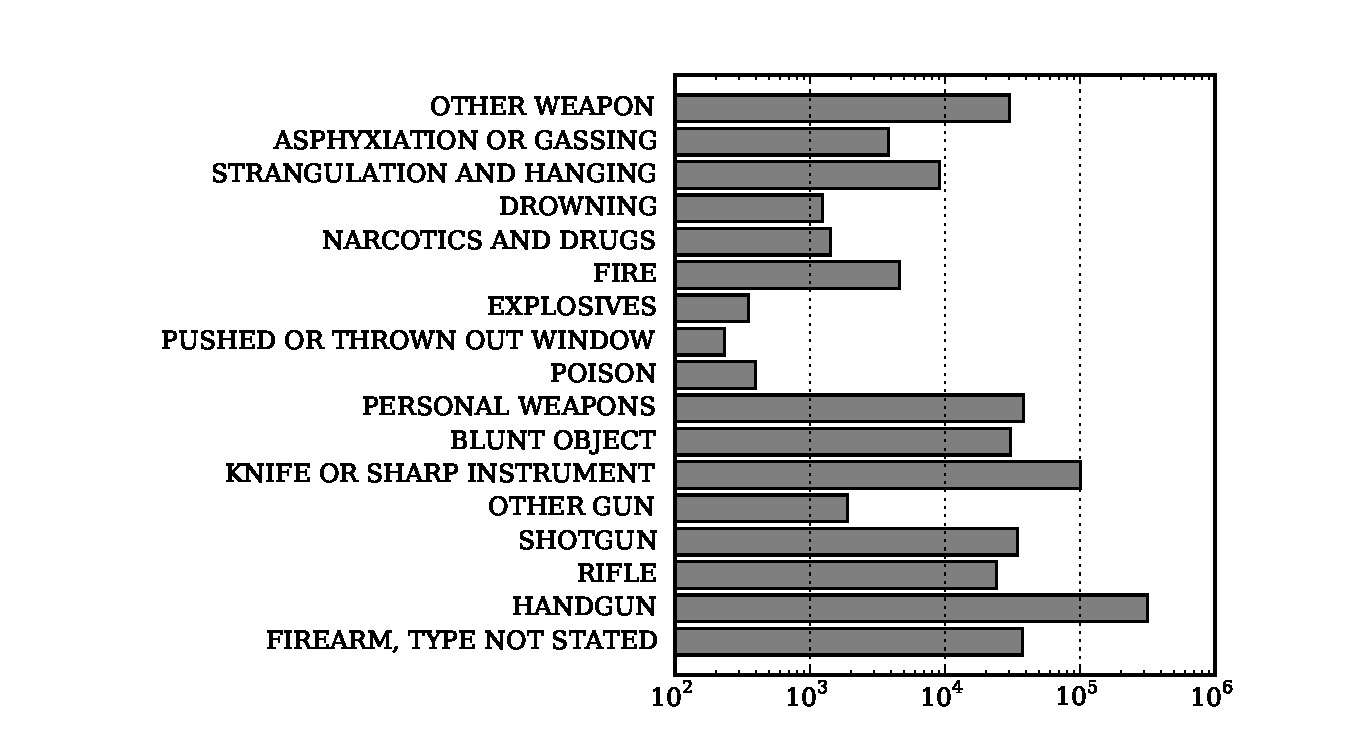
\includegraphics[width=1.0\linewidth]{images/weaps.pdf}
  \caption{The number of deaths from 1976 to 2012 by weapon type.}
  \label{fig_weaps}
\end{figure}

Interesting patterns also exist for the relationship of the victim to the offender (\cref{fig_relationship}).
It turns out that there are many more instances of male offenders killing their female partners, be they wives or girlfriends, with many choosing to murder their past or present significant other with a firearm of some type.
It could be hypothesized that these crimes of passion may be diminished by reducing the immediate access to firearms.

\begin{figure}[H]
  \centering
    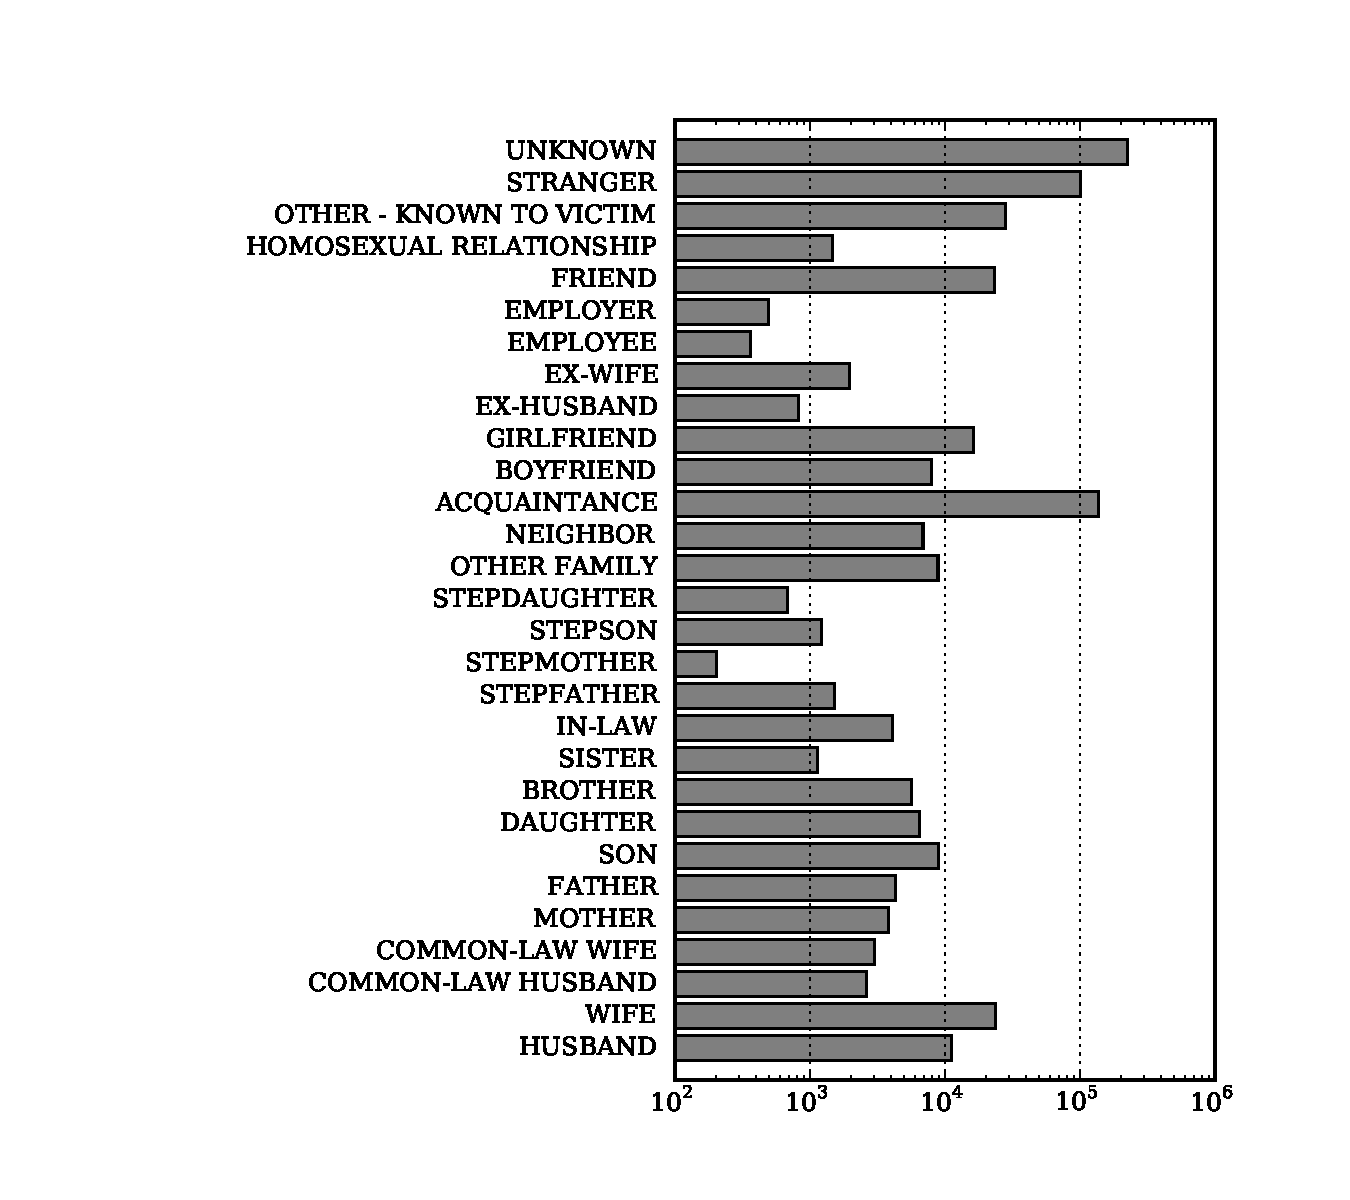
\includegraphics[width=1.0\linewidth]{images/relationship.pdf}
  \caption{The number of deaths from 1976 to 2012 by the relationship of the victim to the offender.}
  \label{fig_relationship}
\end{figure}

The circumstance dimension contains an entry to indicate a justifiable homicide.
In \cref{fig_circumstance} we can see that many of these successful acts of self defense are achieved with the use of a handgun, indicating that these types of firearms may decrease your chances of being brutalized in some way.
Note that no data exists for number of cases of murder in the act of self defense with a firearm, and as such we cannot conclude quantitatively that this theory is correct.

\begin{figure}[H]
  \centering
    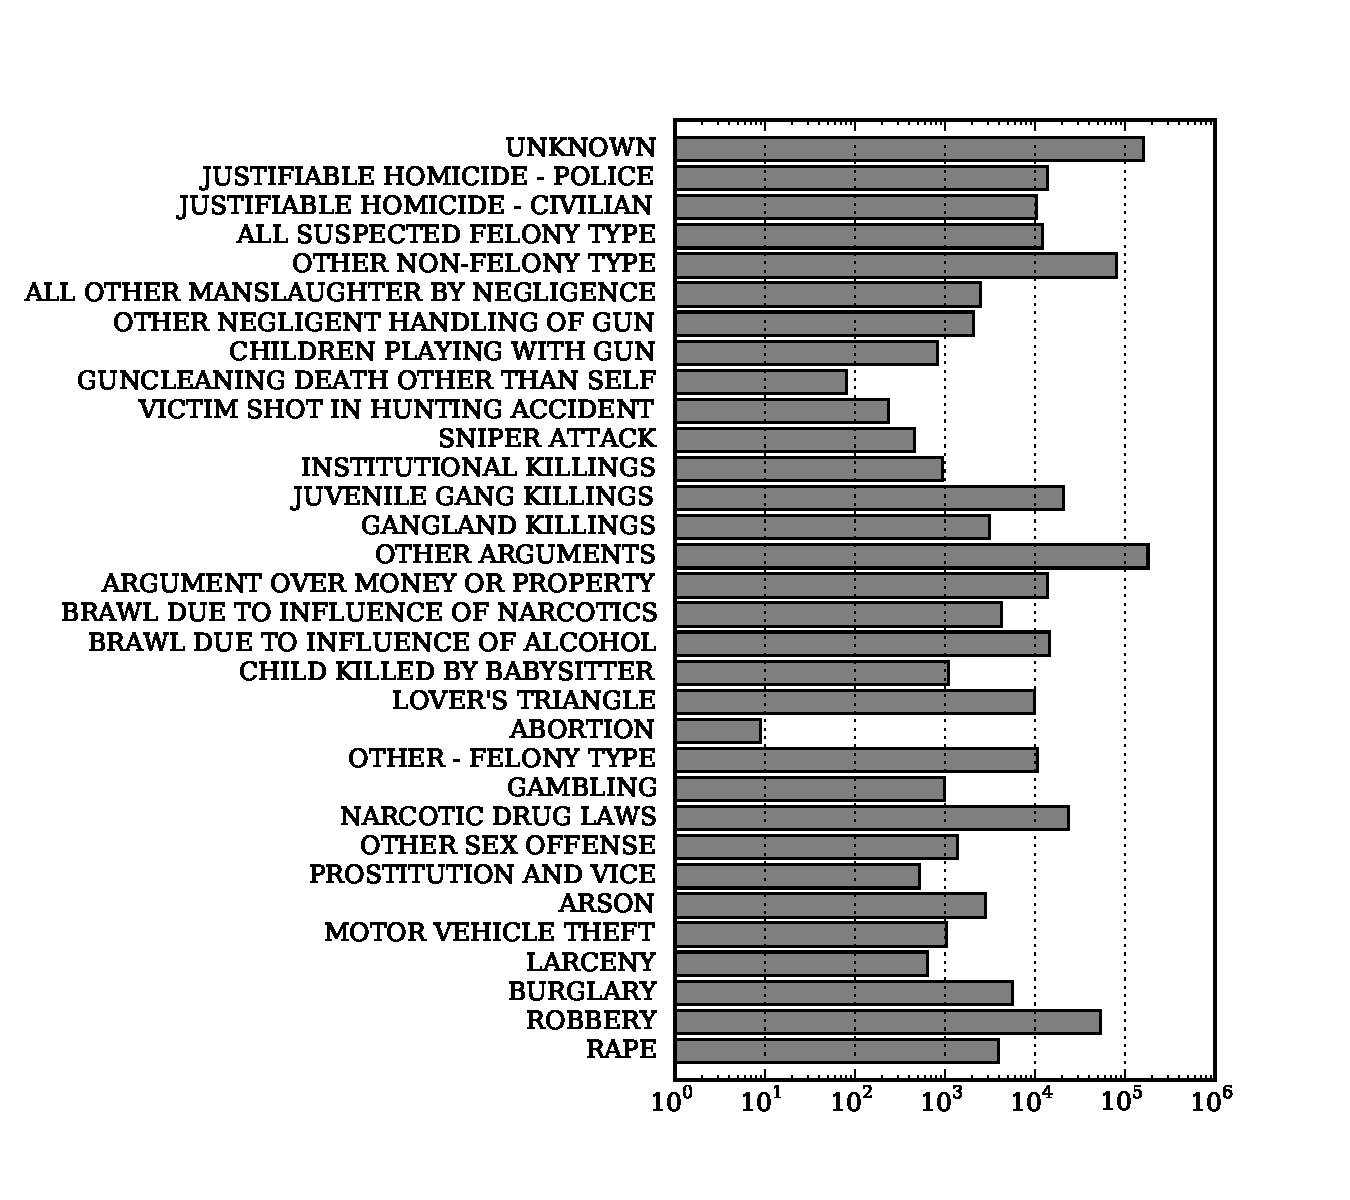
\includegraphics[width=\linewidth]{images/circumstance.pdf}
  \caption{The number of deaths from 1976 to 2012 by homicide circumstance.}
  \label{fig_circumstance}
\end{figure}

\begin{figure*}
  \centering
    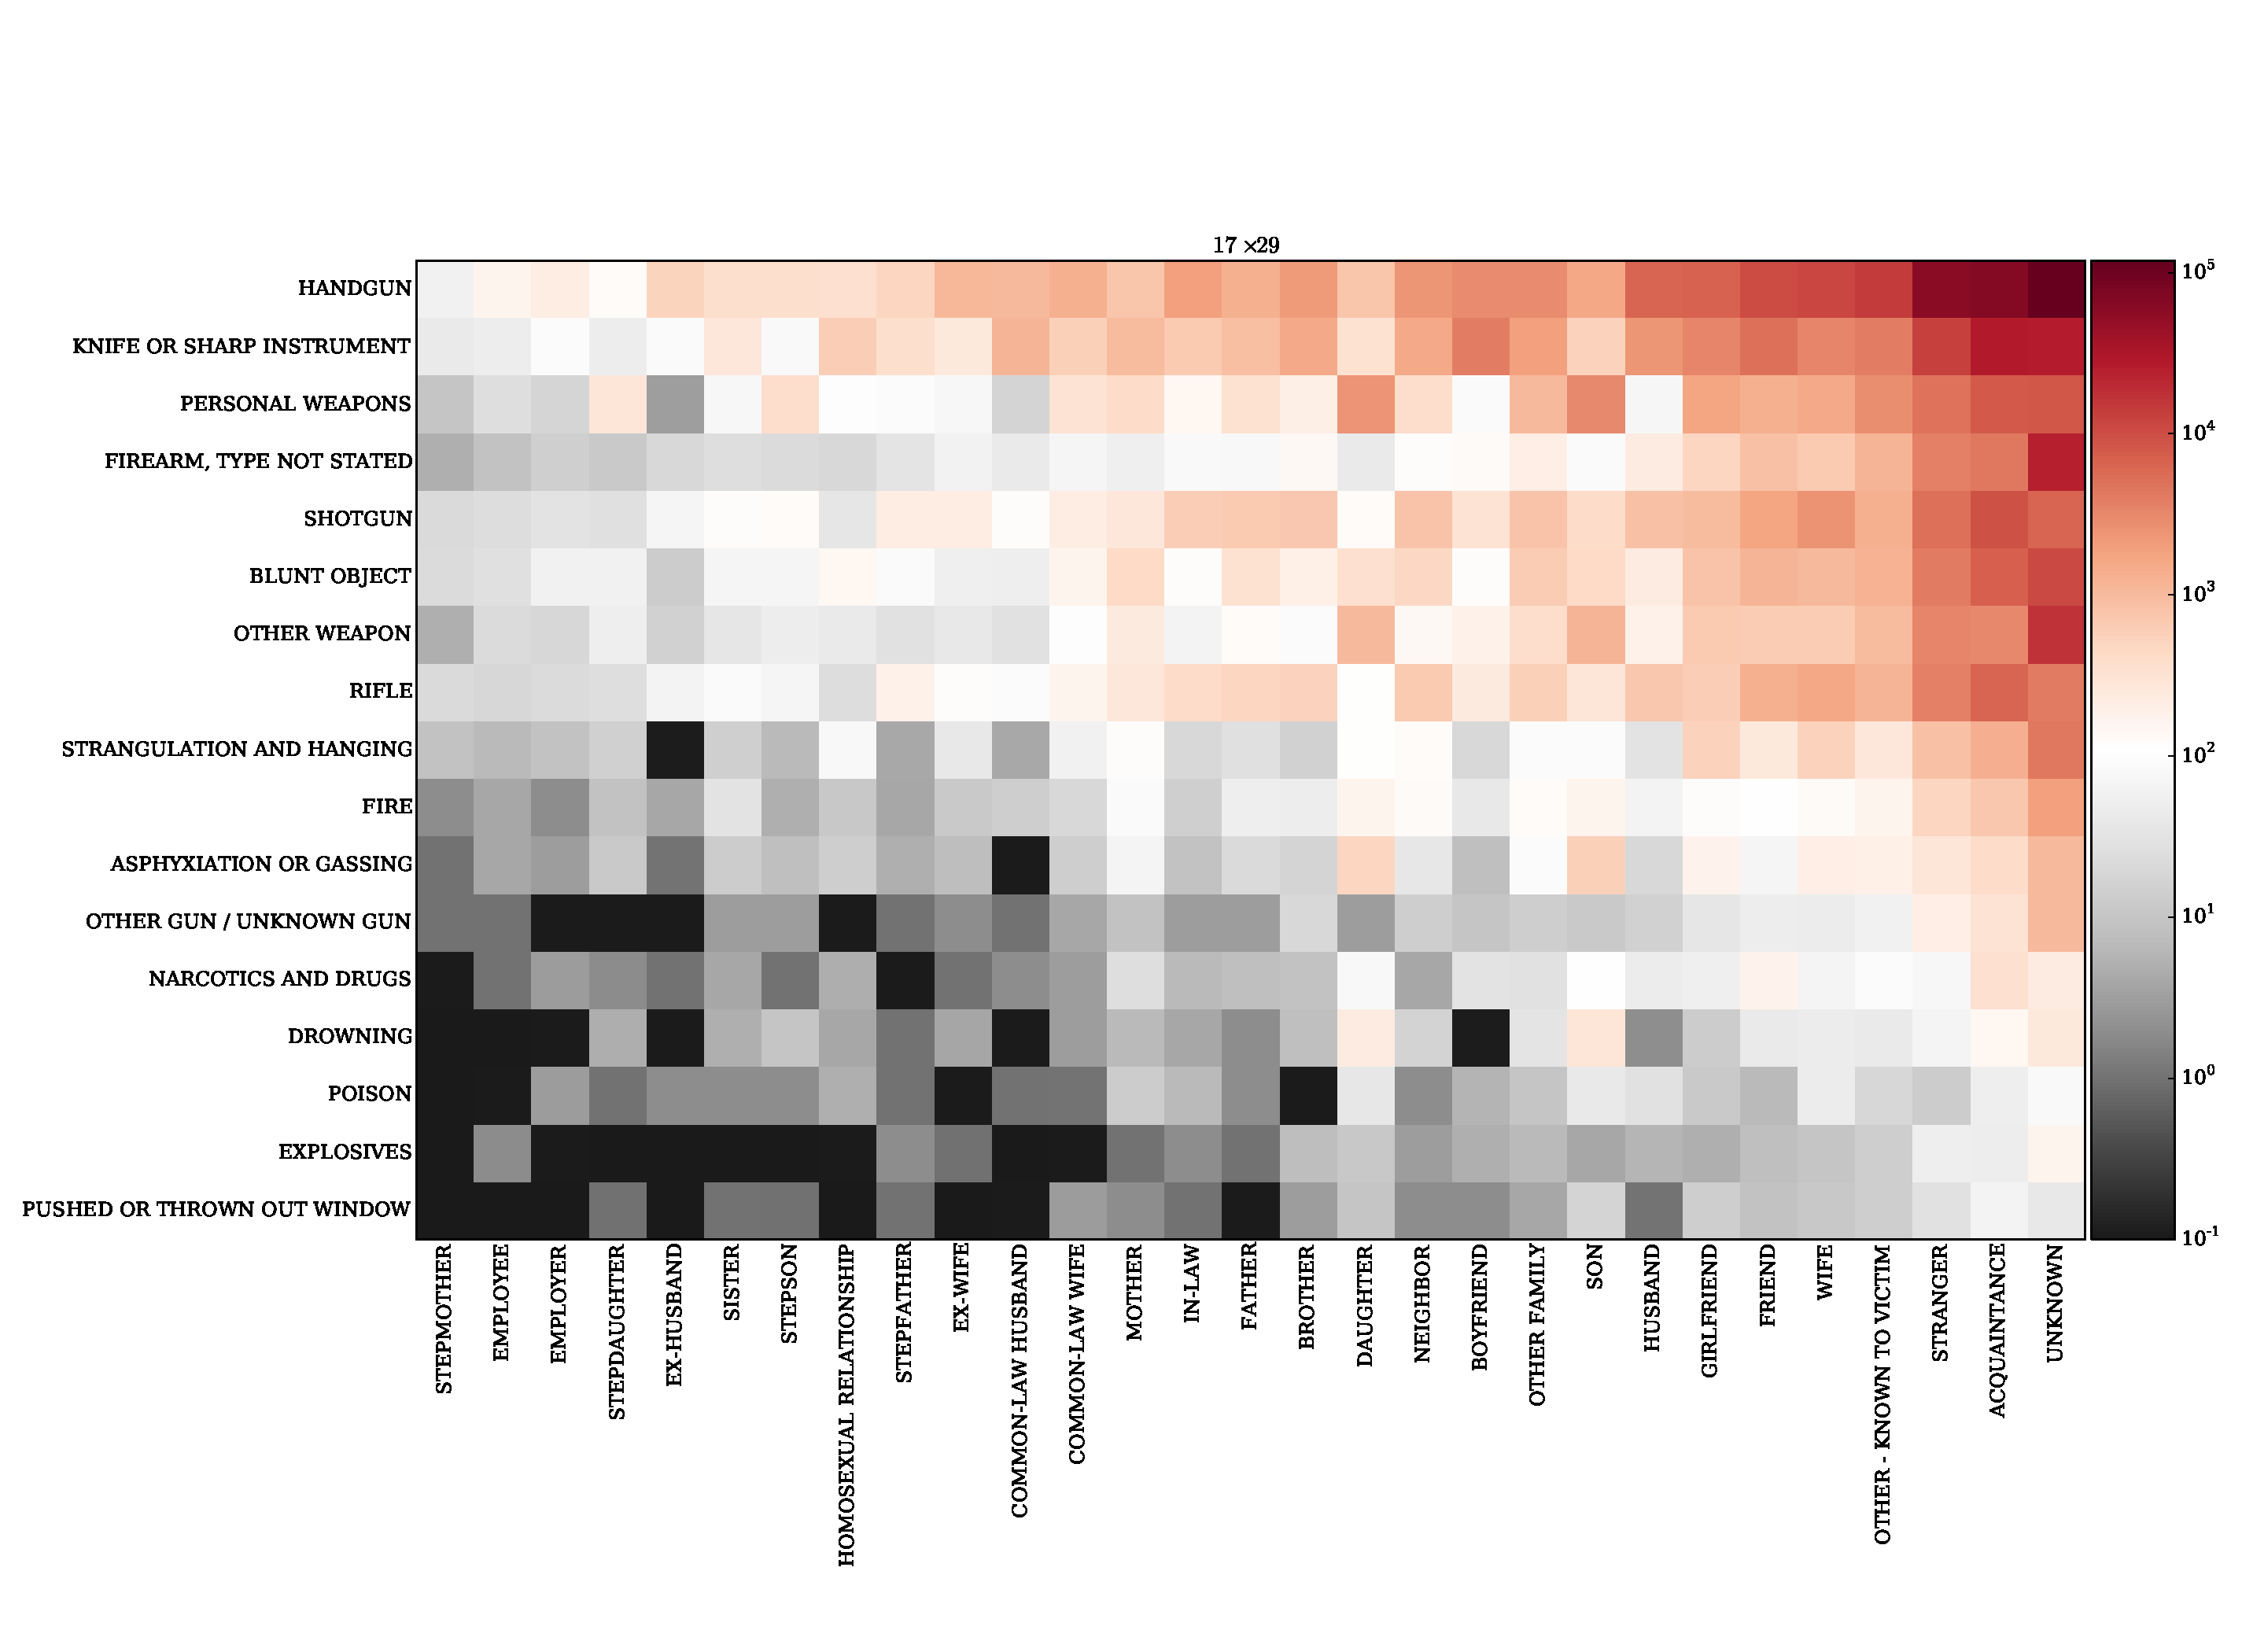
\includegraphics[width=0.8\linewidth]{images/all_data_relation.pdf}
    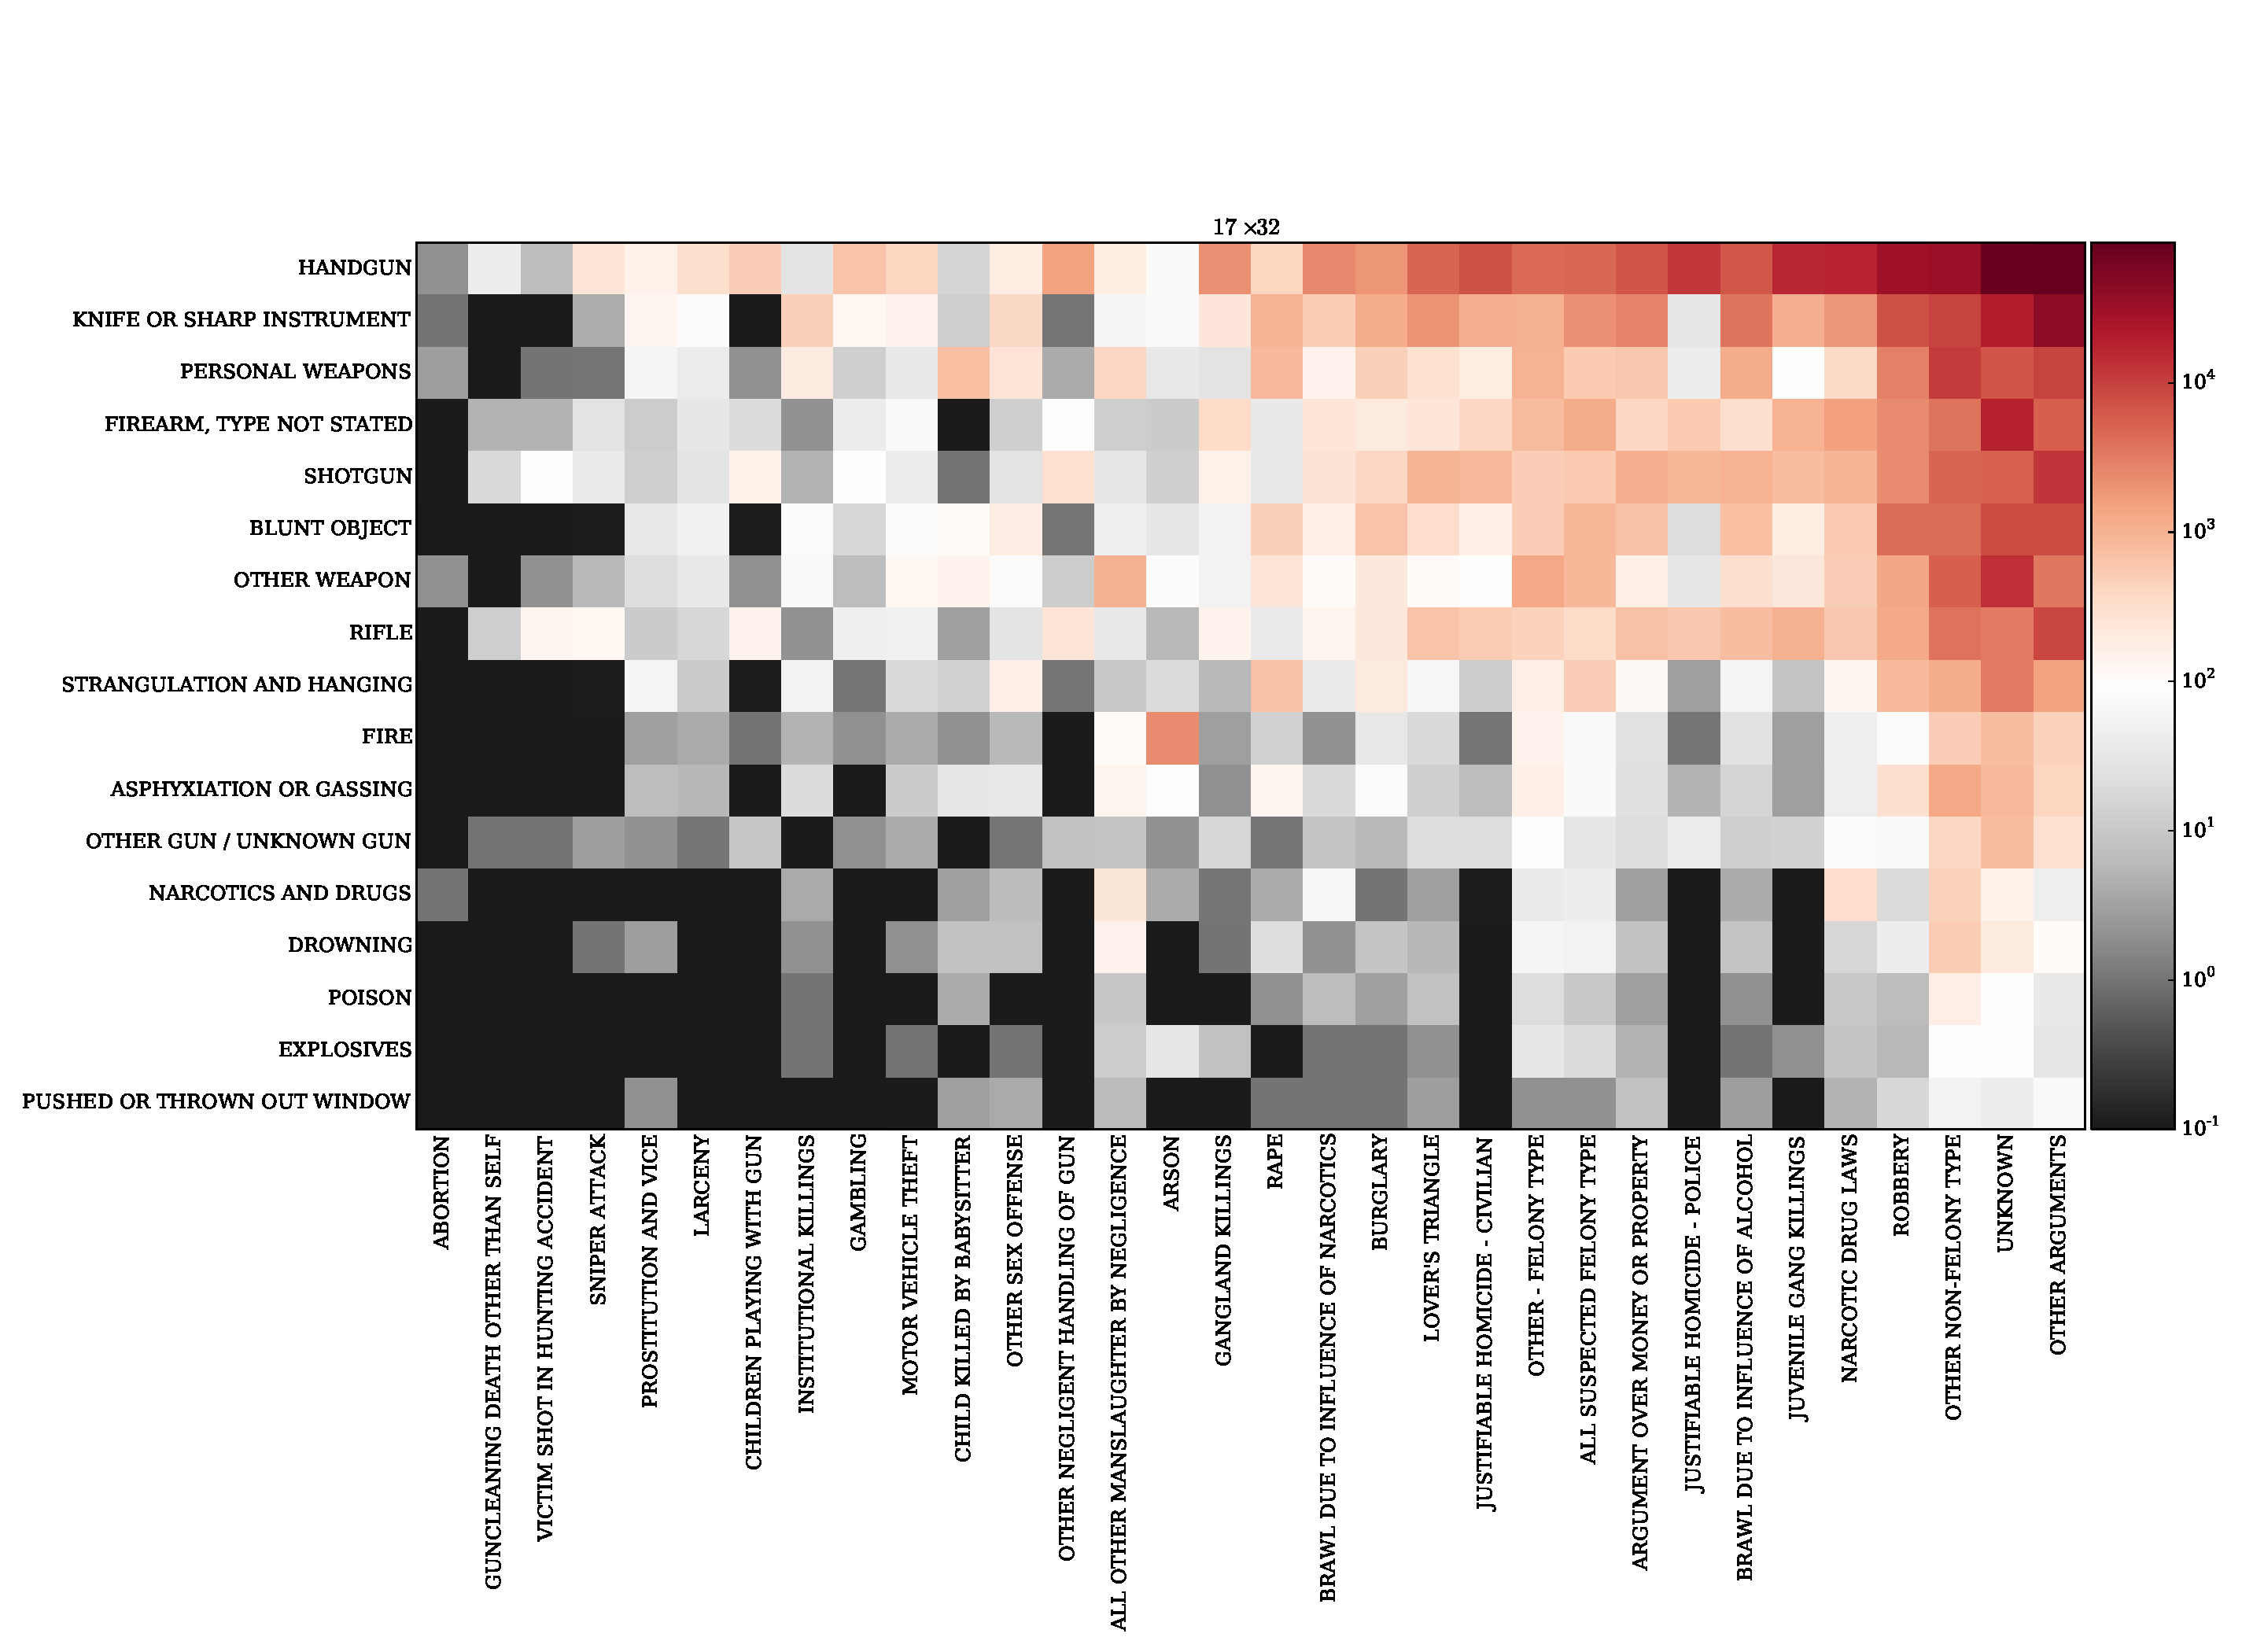
\includegraphics[width=0.8\linewidth]{images/all_data_circum.pdf}
  \caption{Circumstance of 1st offender vs.~weapon used (top) and Relationship of victim to the 1st offender vs.~weapon used (bottom).}
\end{figure*}

\section{Results} \label{sec_results}

To begin, any data rows with missing victim age, victim sex, offender age, or offender sex are eliminated.
The following sections highlight the results from PCA over the whole dataset and LDA with select columns of the data used as classifiers.

The columns of the design matrix are:

\begin{itemize}
  \item year
  \item month
  \item state
  \item group
  \item population
  \item MSA indication
  \item MSA code
  \item type of homicide
  \item situation
  \item victim count
  \item offender count
  \item victim 1 age
  \item victim 1 sex
  \item offender 1 age
  \item offender 1 sex
  \item victim 1 relationship to victim 1
  \item offender 1 circumstance
  \item offender 1 sub-circumstance
\end{itemize}

Because each of these variables are discrete, an integer proxy was used to discriminate between variables.

\subsection{Principle component analysis} \label{sec_pca}

The data are plotted on the two axes of greatest variation in \cref{fig_pca}.

\begin{figure}[H]
  \centering
    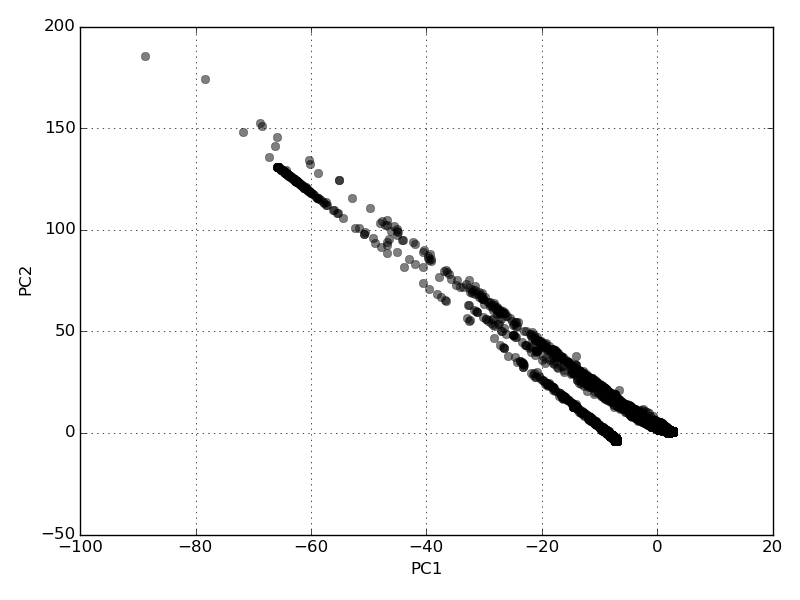
\includegraphics[width=\linewidth]{images/PCA.png}
  \caption{Principle component analysis for the reduced data.  Note the distinct linear trends in the data; these could be distinct clusters of data which could be used to classify the data, or an artifact of using numerical replacement of discrete data.}
  \label{fig_pca}
\end{figure}

\subsection{Linear discriminant analysis} \label{sec_lda}

Linear discriminant analysis finds the axes or axis of greatest variation between a set of classifiers.
In this section the different dimensions of the SHR data are used as classes and the data are plotted on the resulting best-separated axes.

\subsubsection{The ``gun'' class} \label{sec_gun_class}

\begin{figure}[H]
  \centering
    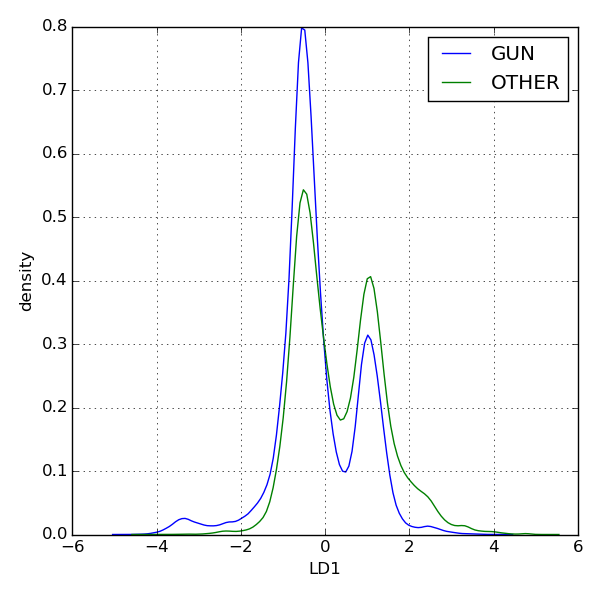
\includegraphics[width=\linewidth]{images/gun/gun.png}
  \caption{Linear discriminant analysis for classes of crimes committed with a gun (blue) and without a gun (green).  The distributions here seem to be very similar, suggesting that the use of a gun in either justifiable or non-justifiable murder follow similar distributions as those committed without.}
  \label{fig_gun}
\end{figure}

\subsubsection{The ``homicide type'' class} \label{sec_homicide_class}

\begin{figure}[H]
  \centering
    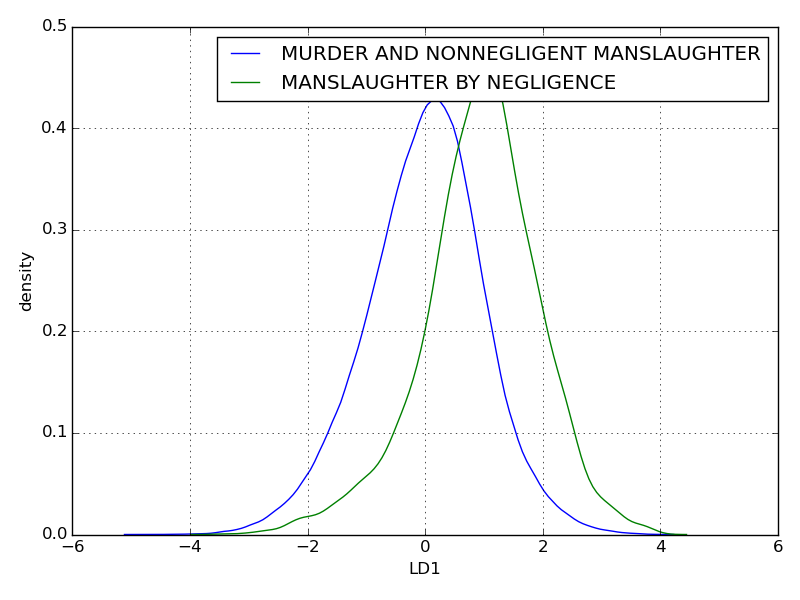
\includegraphics[width=\linewidth]{images/homicide/type.png}
  \caption{Linear discriminant analysis for class based on homicide type, either murder by non-negligent manslaughter (blue) or manslaughter by negligence (green).  It appears that there may be significant differences between these different types of murder.}
  \label{fig_type}
\end{figure}

\subsubsection{The ``offender sex'' class} \label{sec_offender_sex_class}

\begin{figure}[H]
  \centering
    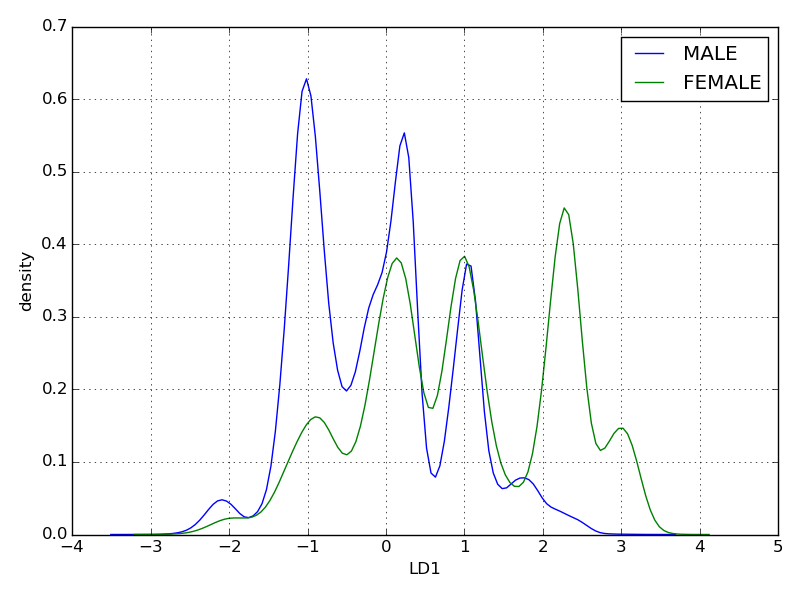
\includegraphics[width=\linewidth]{images/offn_sex/offn_sex.png}
  \caption{Linear discriminant analysis for class based on offender sex with distributions for male (blue) and female (green).  The data is multi-modal, with male clusters skewed left and female clusters skewed right.  There seems to be a significant difference between murders committed by males and females.}
  \label{fig_offn_sex}
\end{figure}

\subsubsection{The ``victim sex'' class} \label{sec_victim_sex_class}

\begin{figure}[H]
  \centering
    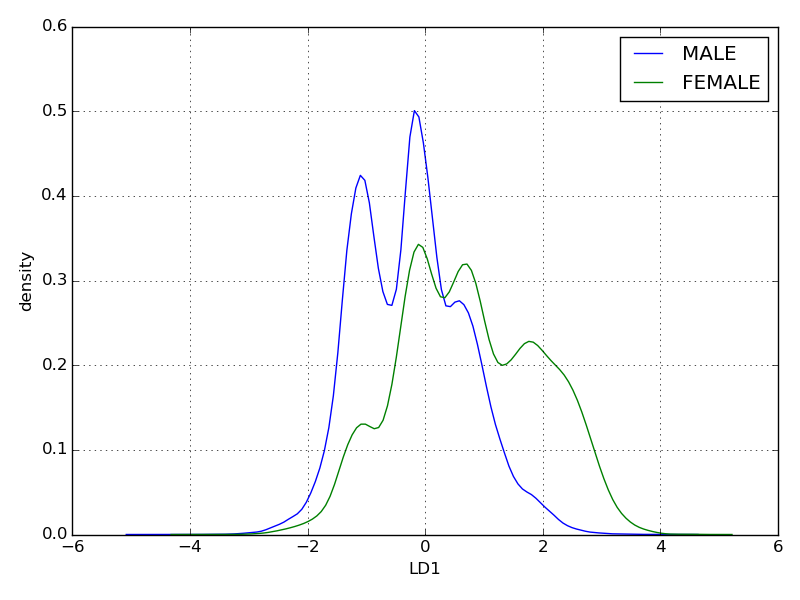
\includegraphics[width=\linewidth]{images/vict_sex/vict_sex.png}
  \caption{Linear discriminant analysis for class based on victim sex with distributions for male (blue) and female (green).  The distributions seem separated enough to be significant.}
  \label{fig_vict_sex}
\end{figure}

\subsubsection{The ``suburban'' class}

\begin{figure}[H]
  \centering
    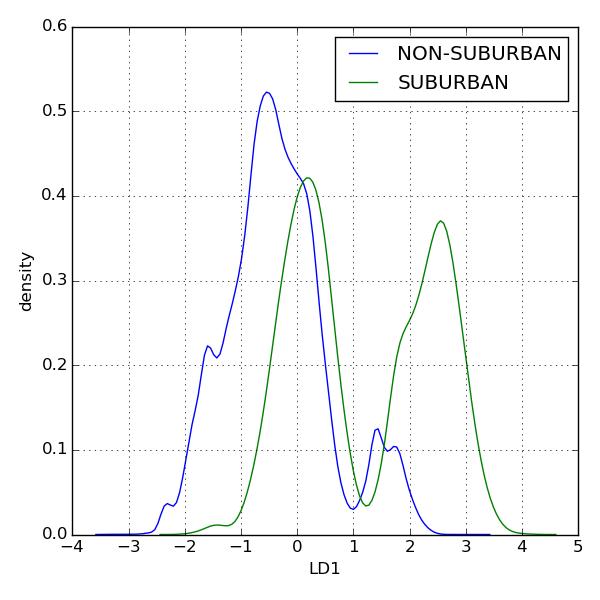
\includegraphics[width=\linewidth]{images/suburban/suburban.png}
  \caption{Linear discriminant analysis with classes defined as suburban (green) and non-suburban (blue) environments.  These data appear bi-modal, with suburban environment deaths exhibiting a remarkable peak on the positive axis.}
  \label{fig_suburban}
\end{figure}

\subsubsection{The ``sub-circumstance'' class}

\begin{figure}[H]
  \centering
  \begin{minipage}[b]{0.30\linewidth}
    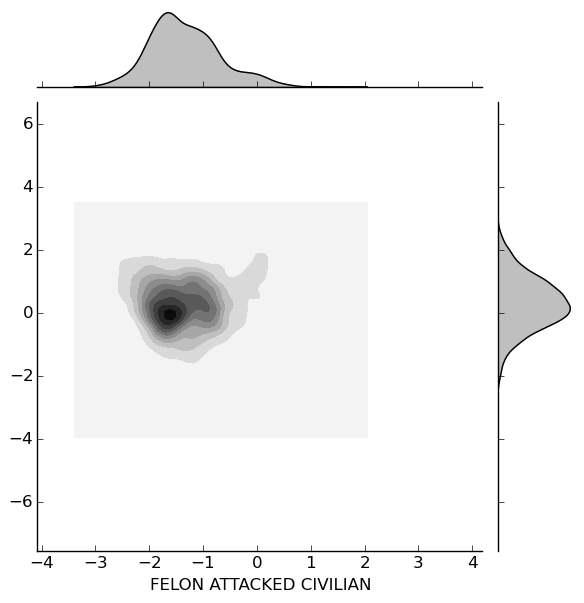
\includegraphics[width=\linewidth]{images/subcircum/FELON_ATTACKED_CIVILIAN.png}
  \end{minipage}
  \quad
  \begin{minipage}[b]{0.30\linewidth}
    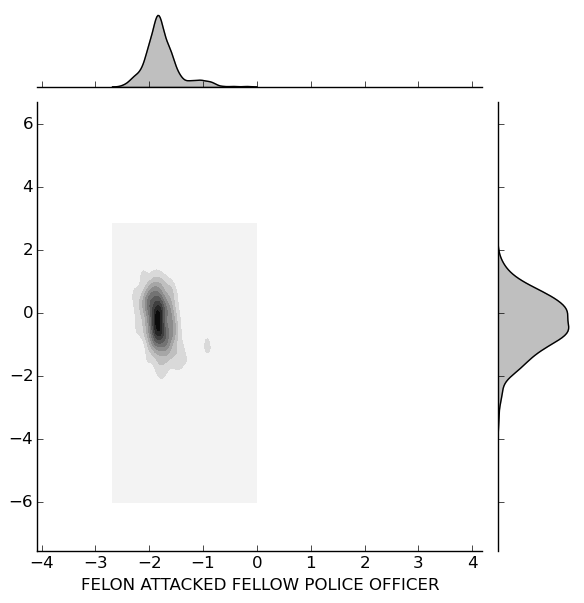
\includegraphics[width=\linewidth]{images/subcircum/FELON_ATTACKED_FELLOW_POLICE_OFFICER.png}
  \end{minipage}
  \quad
  \begin{minipage}[b]{0.30\linewidth}
    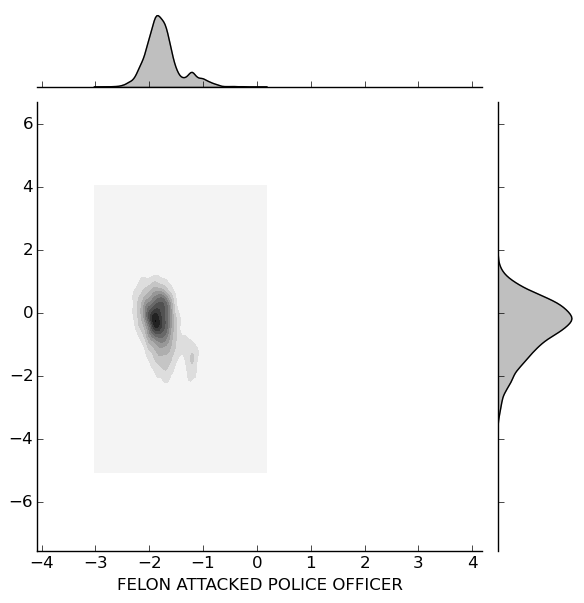
\includegraphics[width=\linewidth]{images/subcircum/FELON_ATTACKED_POLICE_OFFICER.png}
  \end{minipage}

  \begin{minipage}[b]{0.30\linewidth}
    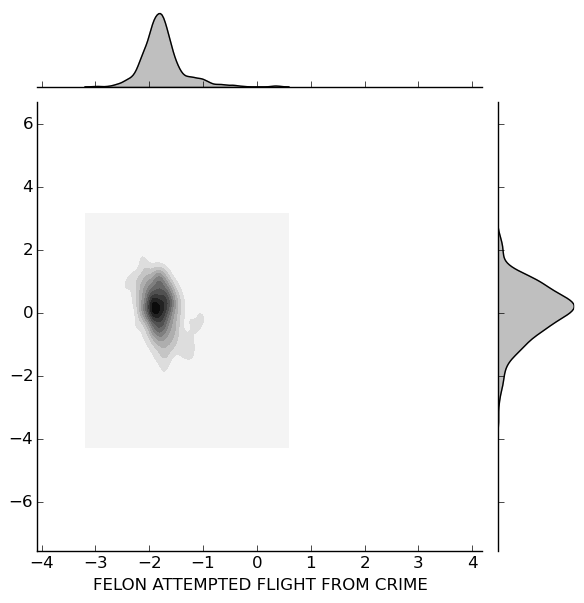
\includegraphics[width=\linewidth]{images/subcircum/FELON_ATTEMPTED_FLIGHT_FROM_CRIME.png}
  \end{minipage}
  \quad
  \begin{minipage}[b]{0.30\linewidth}
    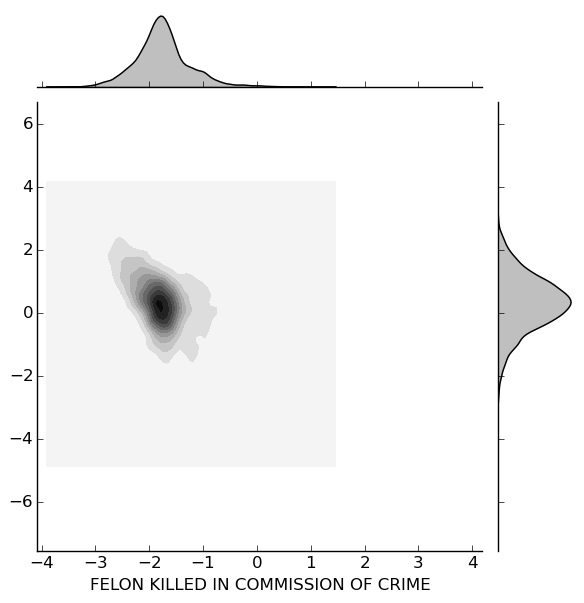
\includegraphics[width=\linewidth]{images/subcircum/FELON_KILLED_IN_COMMISSION_OF_CRIME.png}
  \end{minipage}
  \quad
  \begin{minipage}[b]{0.30\linewidth}
    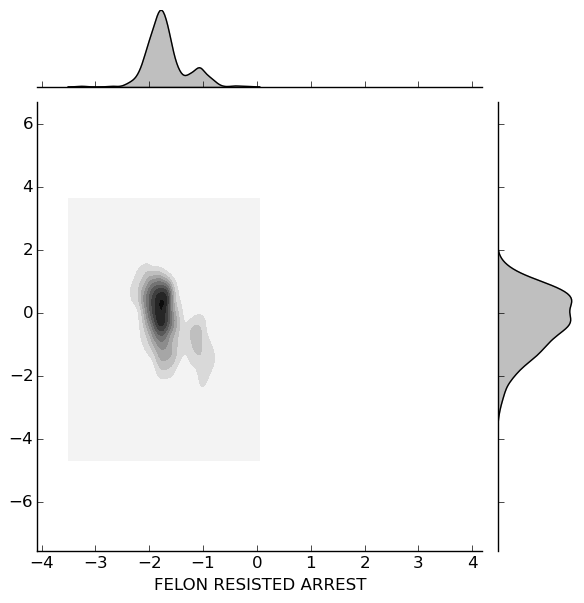
\includegraphics[width=\linewidth]{images/subcircum/FELON_RESISTED_ARREST.png}
  \end{minipage}
  \caption{Results of linear discriminant analysis with classes defined as sub-circumstances of the death.  There were two significant linear discriminants, depicted here with the x- and y-axes with distributions for each discriminant depicted in the upper and right sides respectively.  The mean of each of the distributions are close to (-2,0), and some of the class types' x-axes show a weak-bi-modal distribution.}
  \label{fig_sub_circumstance}
\end{figure}

\subsubsection{The ``weapon'' class}

\begin{figure}[H]

  \centering

  \begin{minipage}[b]{0.20\linewidth}
    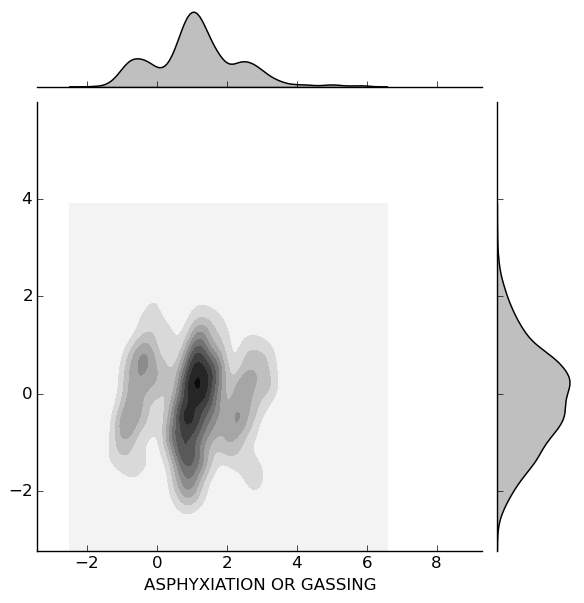
\includegraphics[width=\linewidth]{images/weapon/ASPHYXIATION.png}
  \end{minipage}
  \quad
  \begin{minipage}[b]{0.20\linewidth}
    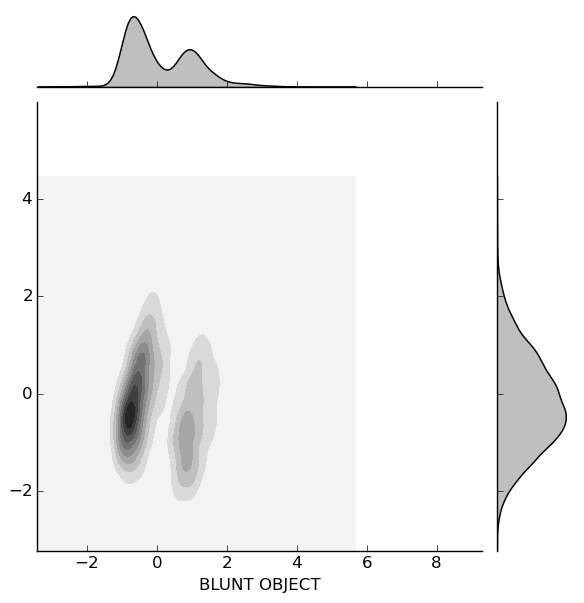
\includegraphics[width=\linewidth]{images/weapon/BLUNT_OBJECT.png}
  \end{minipage}
  \quad
  \begin{minipage}[b]{0.20\linewidth}
    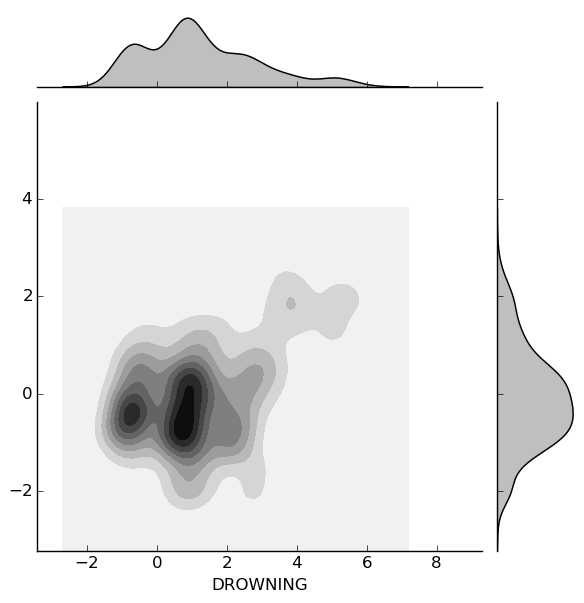
\includegraphics[width=\linewidth]{images/weapon/DROWNING.png}
  \end{minipage}
  \quad
  \begin{minipage}[b]{0.20\linewidth}
    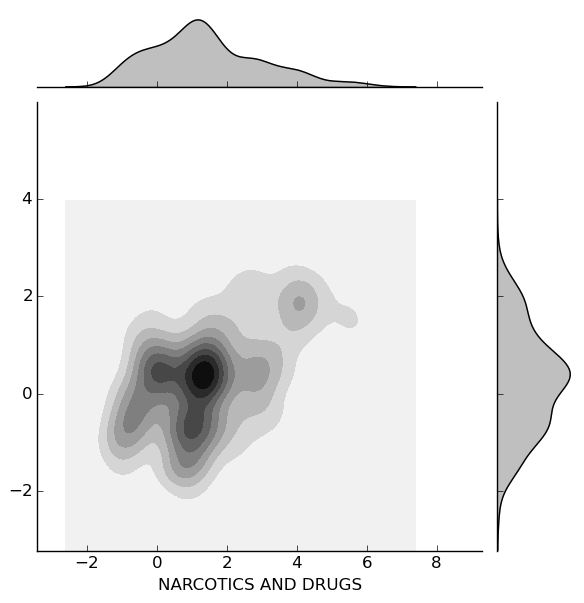
\includegraphics[width=\linewidth]{images/weapon/DRUGS.png}
  \end{minipage}

  \begin{minipage}[b]{0.20\linewidth}
    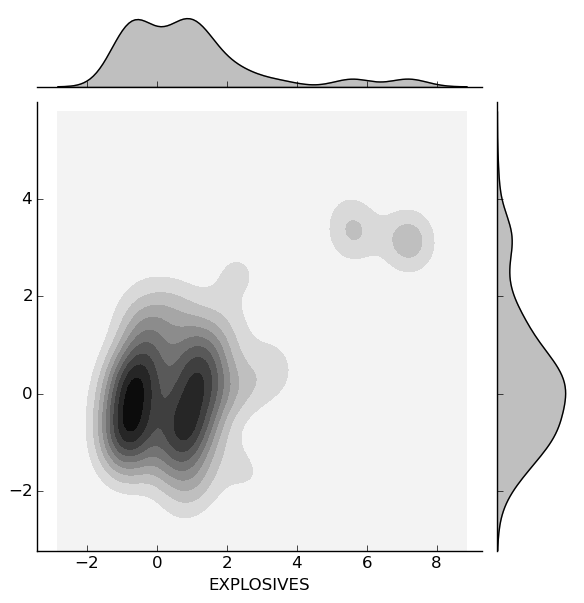
\includegraphics[width=\linewidth]{images/weapon/EXPLOSIVES.png}
  \end{minipage}
  \quad
  \begin{minipage}[b]{0.20\linewidth}
    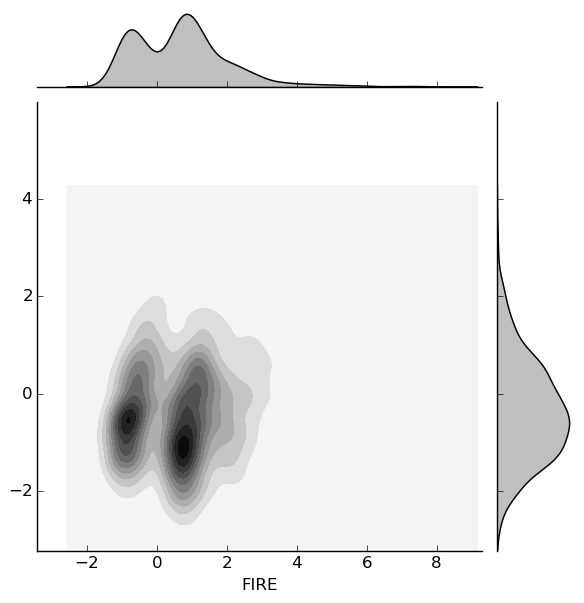
\includegraphics[width=\linewidth]{images/weapon/FIRE.png}
  \end{minipage}
  \quad
  \begin{minipage}[b]{0.20\linewidth}
    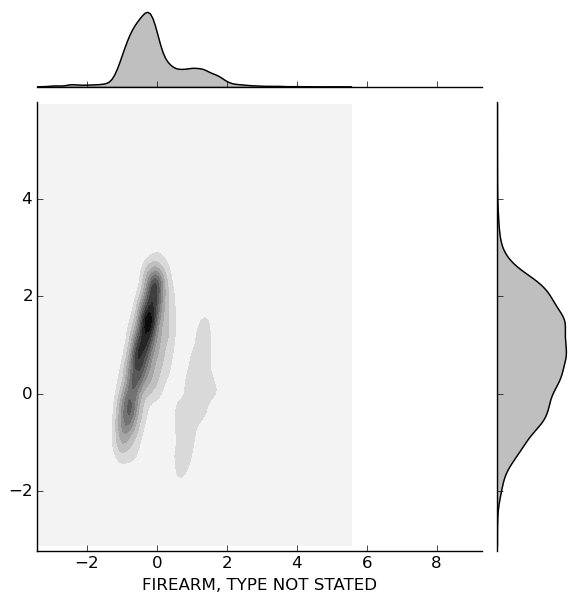
\includegraphics[width=\linewidth]{images/weapon/FIREARM_TYPE_NOT_STATED.png}
  \end{minipage}
  \quad
  \begin{minipage}[b]{0.20\linewidth}
    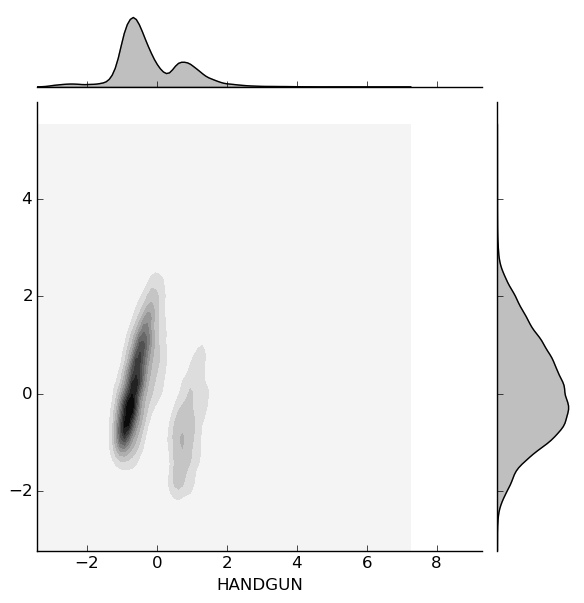
\includegraphics[width=\linewidth]{images/weapon/HANDGUN.png}
  \end{minipage}

  \begin{minipage}[b]{0.20\linewidth}
    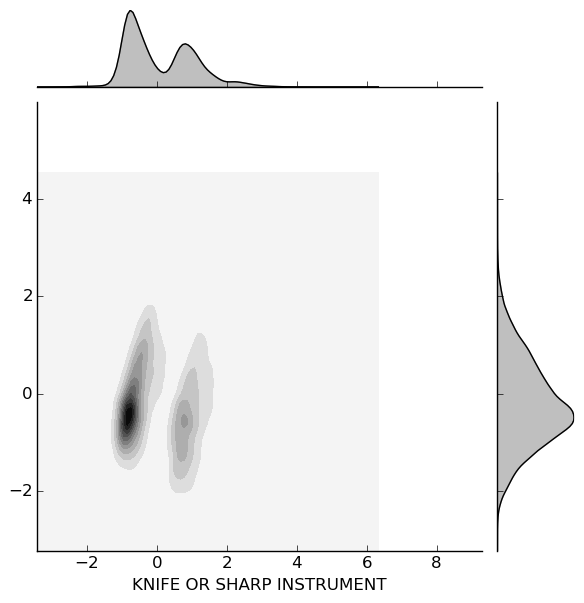
\includegraphics[width=\linewidth]{images/weapon/KNIFE.png}
  \end{minipage}
  \quad
  \begin{minipage}[b]{0.20\linewidth}
    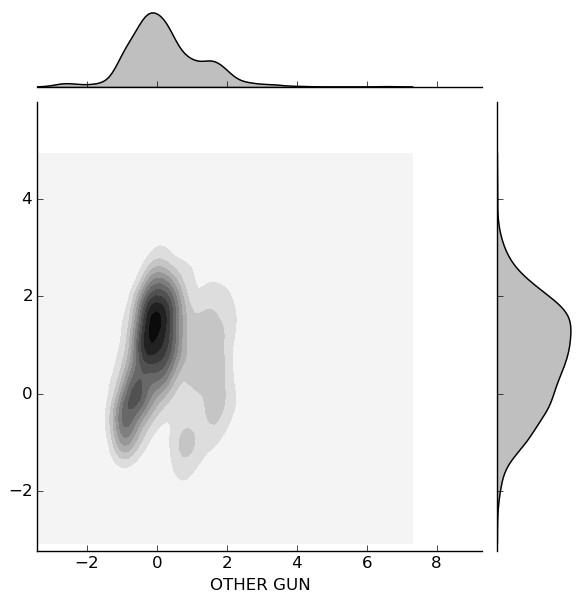
\includegraphics[width=\linewidth]{images/weapon/OTHER_GUN.png}
  \end{minipage}
  \quad
  \begin{minipage}[b]{0.20\linewidth}
    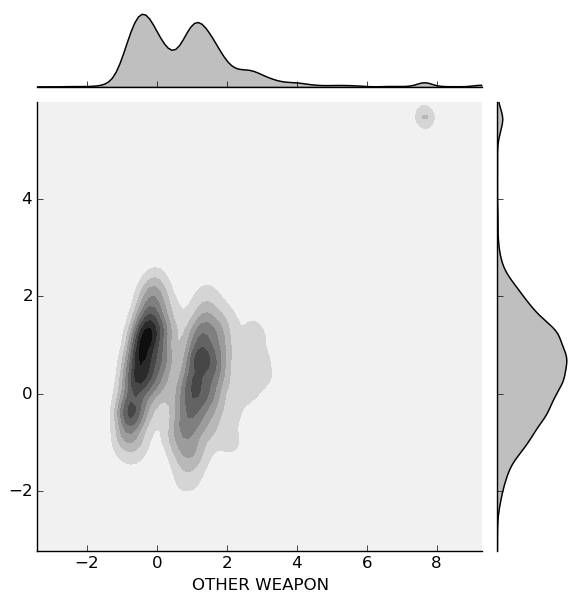
\includegraphics[width=\linewidth]{images/weapon/OTHER_WEAPON.png}
  \end{minipage}
  \quad
  \begin{minipage}[b]{0.20\linewidth}
    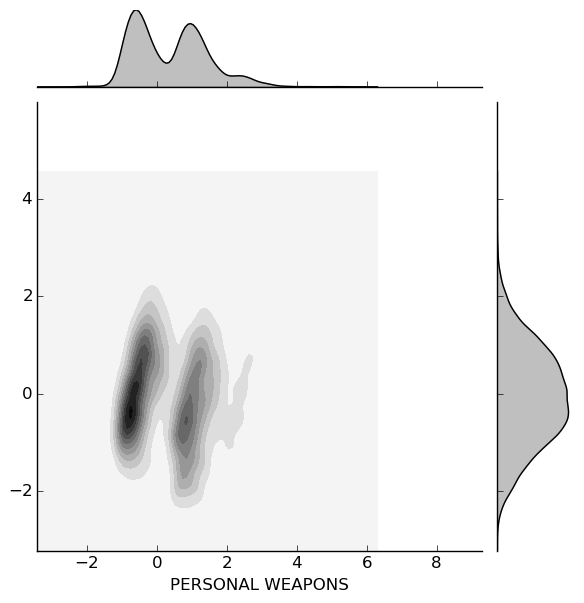
\includegraphics[width=\linewidth]{images/weapon/PERSONAL_WEAPONS.png}
  \end{minipage}

  \begin{minipage}[b]{0.20\linewidth}
    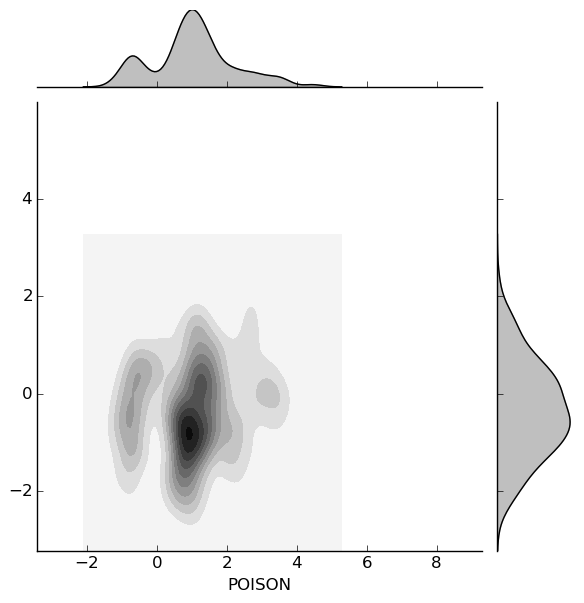
\includegraphics[width=\linewidth]{images/weapon/POISON.png}
  \end{minipage}
  \quad
  \begin{minipage}[b]{0.20\linewidth}
    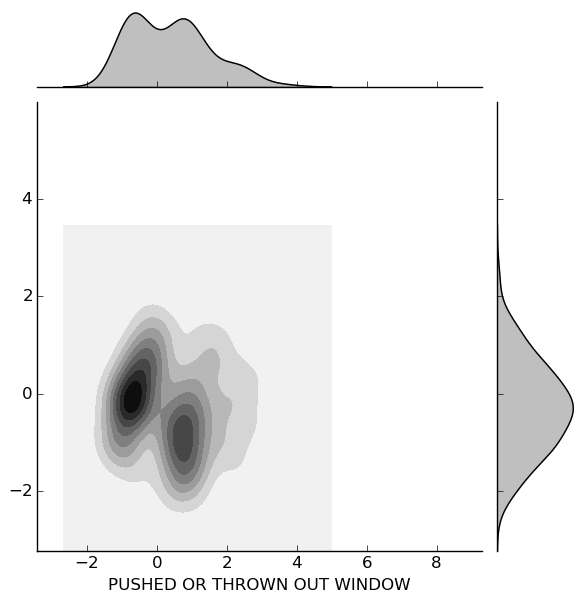
\includegraphics[width=\linewidth]{images/weapon/PUSHED_OUT_WINDOW.png}
  \end{minipage}
  \quad
  \begin{minipage}[b]{0.20\linewidth}
    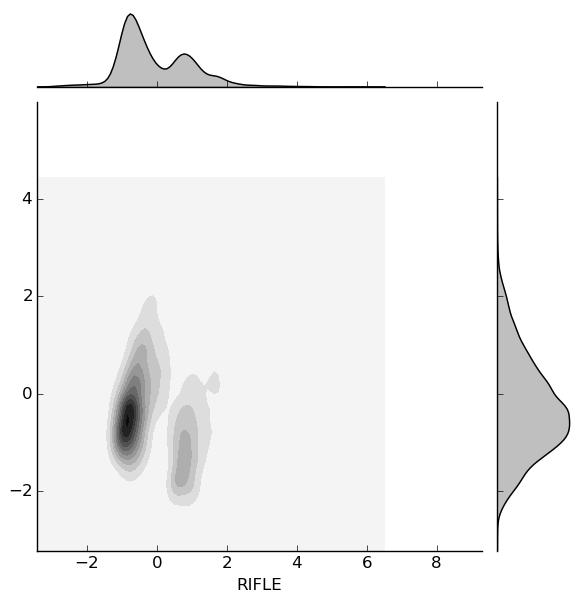
\includegraphics[width=\linewidth]{images/weapon/RIFLE.png}
  \end{minipage}
  \quad
  \begin{minipage}[b]{0.20\linewidth}
    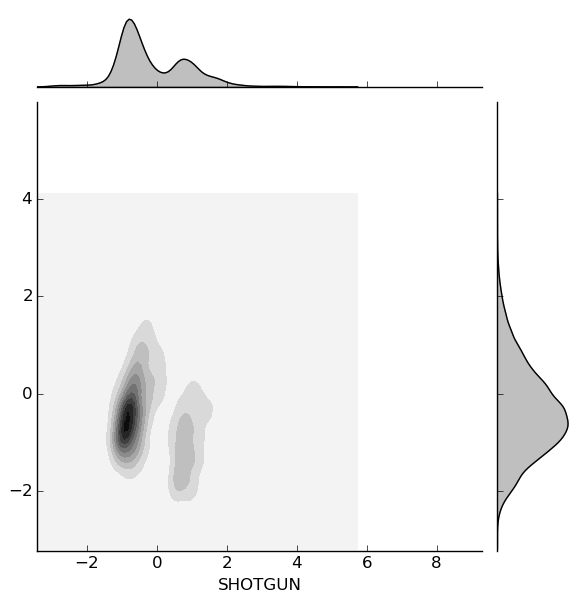
\includegraphics[width=\linewidth]{images/weapon/SHOTGUN.png}
  \end{minipage}

  \begin{minipage}[b]{0.20\linewidth}
    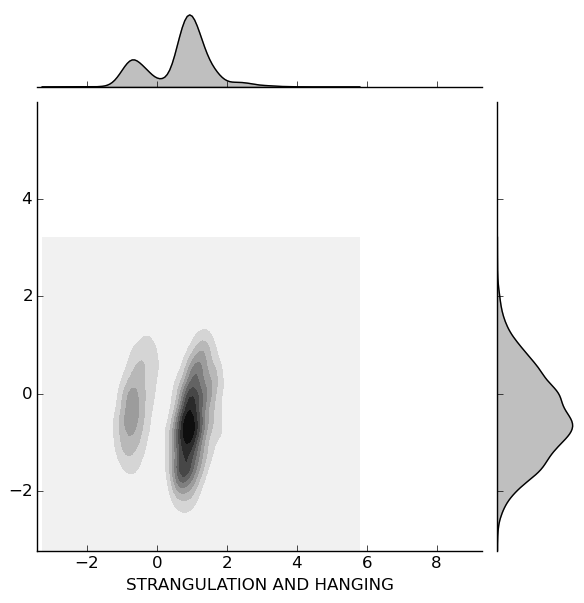
\includegraphics[width=\linewidth]{images/weapon/STRANGULATION.png}
  \end{minipage}
  \quad
  \begin{minipage}[b]{0.20\linewidth}
    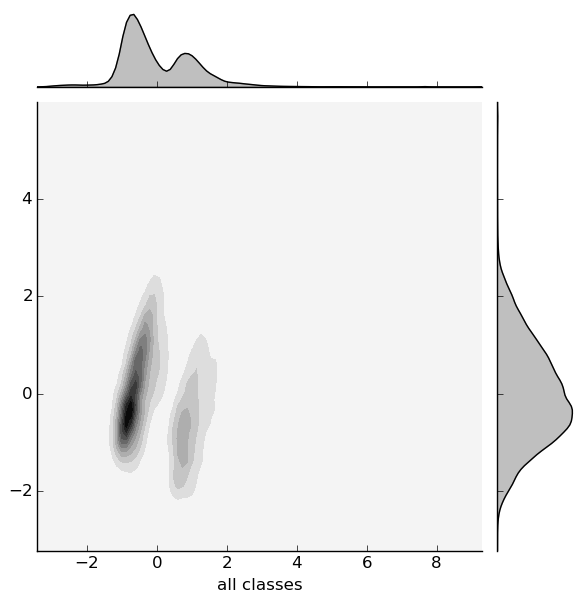
\includegraphics[width=\linewidth]{images/weapon/all.png}
  \end{minipage}

  \caption{Results of linear discriminant analysis with weapon type class.  There were two significant linear discriminants, depicted here with the x- and y-axes with distributions for each discriminant depicted in the upper and right sides respectively.  Many classes of weapons display tri- and bi-modal distributions in the x-axis discriminant.}
  \label{fig_weap_type}

\end{figure}

\newpage

\section{Discussion}

While the PCA results are inconclusive, the LDA results indicate that some of the ``classes'' described in \cref{sec_results} may be used to categorize homicides.
A non-parametric test, such has Wilcoxon, might be used to determine significance for classifying by gun and non-gun murders (\cref{fig_gun}).
However, there is a very clear separation between murders and manslaughter by negligence (\cref{fig_type}) and suburban and non-suburban environments (\cref{fig_suburban}).
Furthermore, the offender and victim sex, sub-circumstance, and weapon type classes provide some degree of separation (\cref{fig_offn_sex,fig_vict_sex,fig_sub_circumstance,fig_weap_type}).
This suggests that a higher-order analysis of the data, supplemented with additional explanatory variables, may provide some insight into the nature of violence in the US.
Finally, an identical analysis to that presented here performed over each year in the data individually may isolate any time-dependent characteristics of the data.

\section{Conclusion}

Some interesting patterns have emerged from this stud which suggest that a further exploration of the FBI dataset may be fruitful.
If successful, this project may be used to evaluate crime in a region and derive an appropriate gun-control law.
It may be possible to substantially reduce gun-violent-death.
At the very least this study will provide new insight into the nature of violent death in the U.S., as well as the complicated relationships between the offenders and their victims.

\printbibliography

%\begin{figure}[H]
%  \centering
%    \includegraphics[width=0.45\textwidth]{images/.png}
%\end{figure}


\end{document}


